% ==========================================================================================
\section{Inferring Release Lines from Gossip}
\label{sec:inference}

\subsection{Release lines}
We built a table of the \texttt{node\_announcement} feature bits of every release of the four implementations from
their source at each release tag: LND 0.7--0.21.4, Core Lightning (CLN) 0.8.2--26.06.9, Eclair 0.3--0.14.3 and LDK
0.0.113--0.2.7. For each release we record the bits it sets by default, the bits an operator can add through
options, flags, plugins or known custom extensions, and the default bits an operator can switch off; each entry
cites the source file it comes from. A release's date is its publication date (GitHub release page; crates.io for
LDK), the day operators could install it. Consecutive releases with identical defaults form a \emph{release line}, the
finest unit gossip can resolve: LND has 10 lines from 0.8 to 0.21, CLN 13, Eclair 13 and LDK 6. Some lines are
single minor releases (LND 0.18, 0.19, 0.20, 0.21); others span several (LND 0.15.1--0.17; LDK 0.0.120--0.1 covers
January~2024 to December~2025). Patch releases never change the defaults, so a patch level is never visible.

For a node with feature set $B$, a line $\ell$ with defaults $D_\ell$, optional bits $O_\ell$ and removable bits
$R_\ell$ is \emph{consistent} when $D_\ell \setminus R_\ell \subseteq B \subseteq D_\ell \cup O_\ell$. The
\emph{strict range} is every consistent line released by the day of observation; it contains the running line under
any non-developer configuration. The \emph{likely line} is the consistent line that needs the fewest non-default
bits among the lines released by the day the node's current feature set first appeared. Dating the inference to
that day matters: a node cannot run a line that did not exist when it began announcing its bits, and without it a
new release would relabel every node whose existing bits happen to fit the new line (233 CLN nodes running 24.05 with
the onion-message option would have ``upgraded'' to 24.08 on its release day). A set consistent only with lines not
yet released is a pre-release build; a set consistent with no line is unrecognised.

\subsection{Implementation}
Release lines are defined per implementation, so the implementation comes first. We revise the feature-bit rules of
our previous paper~\cite{kumar2026clientdiversity}: LND-only bits (2023, 31) and Eclair-only bits (37, or 29
with 61) are decisive; a set with bits 11 and 39 or 43 is CLN when bit 5 is set and Eclair otherwise; 39, 43 or 63
without 11 is LDK. The CLN--Eclair split now uses bit 5 (\texttt{upfront\_shutdown\_script}), which every CLN
release sets, instead of keysend (bit 55), which operators can switch off. New in this paper, the release table
itself is evidence. When a set is consistent with the
lines of exactly one implementation, that implementation is assigned, which recovers releases older than the
distinguishing bits, such as LND 0.8--0.11 and CLN before 23.05; and when a bit rule names an implementation that
has no release producing the set while exactly one other implementation does, the table wins. Weak signals (LND's
default colour or alias, default CLTV deltas) label the remaining nodes with low confidence, and only operator-attributed
and high-confidence labels receive a release line. Announcements that are not visible on a day (last update~0)
carry the node's previous feature set forward.

\subsection{Validation}
\label{sec:validation}
\paragraph{Implementation}
\NAnchorClient{} nodes name their implementation in their alias (``\ldots{}[LND]'', ``\ldots{}-CLN'', ``eclair'',
``ldk-node''); LND's default alias is excluded because the rules use it. On the latest day each was announced with
channels, the labels reach precision \PrecLND\% and recall \RecLND\% for LND (\NAnchorLND{} nodes) and precision
\PrecCLN\% and recall \RecCLN\% for CLN (\NAnchorCLN{} nodes) (Table~\ref{tab:validation}). The misses are almost
all low-confidence labels, which receive no release line.

\paragraph{Release line}
CLN built in developer mode puts the version into the default alias (e.g.\ \texttt{YELLOWWATER-v25.09}); the alias
follows the binary, so it is correct on every day the node is announced. Over \NVerNodeDays{} announced node-days of
\NVerNodes{} such nodes on \NVerLines{} lines (no operator above \PctVerMaxOperator\% of node-days), the strict range
contains the stated line on \PctVerStrict\% of node-days and the likely line is exact on \PctVerLikely\%
(Fig.~\ref{fig:validation}). Node-days of one node are not independent, so the node is the better unit: of the
\NVerNodeLines{} combinations of node and stated line, \NVerNodeLinesExact{} are exact on every day
(\PctNodeLineExact\%, 95\% CI \NodeLineCILo--\NodeLineCIHi\%). The misses are a 24.05 node with the onion-message
option, which makes it identical to 24.08; a 25.02.1 node and a 23.11.1 node whose switched-off options make them look
one line older; and a single day of a release candidate.

\paragraph{Checks without ground truth}
No LND node in our data states its version in its alias, so for LND, where most of our dynamics are measured, we rely
on checks that a wrong release table would fail. First, operators rarely return to an older release, while a noisy
inference would make nodes flicker between lines: among consecutive observations of live nodes, the likely line
decreases in \PctDownLND\% of line changes for LND (against \NUpLND{} increases) and in \PctDownCLN\% for CLN. Second,
a line assigned the wrong bits would show nodes on it long before its release: each LND line released since 2024 was
seen on at most \PreRelLndMax{} nodes before its publication, against \PostRelLndMin--\PostRelLndMax{} in its first
90~days. Third, a check from outside gossip: a platform that ships a new LND version moves its nodes to a known line
(\S\ref{sec:waves}). Of the \NPlatLineChanges{} line changes whose new announcement was signed within 48~hours after
one of the four platform releases that introduced a new LND line, \PlatLineMin--\PlatLineMax\% landed
on the line that release shipped.

\paragraph{What gossip cannot resolve}
Among live nodes with a release line, the strict range spans more than one line on \PctStrictMultiLND\% of LND and
\PctStrictMultiCLN\% of CLN node-days in 2026, because options let an older line imitate a newer one; the likely line
is unique on all of them. Unrecognised sets are \PctUnrecLND\% (LND) and \PctUnrecCLN\% (CLN) of node-days,
and pre-release builds about \PctPreLND\% of LND node-days. Three limits remain. Patch releases are invisible.
A node that upgrades without restarting, or whose new announcement does not reach us, keeps its old bits. Developer
overrides and forks can imitate any set. The first two bias exposure upward, the third in either direction; none
can be measured from gossip alone, which is why we report the strict and likely ranges side by side.

\begin{figure}[t]
\centering
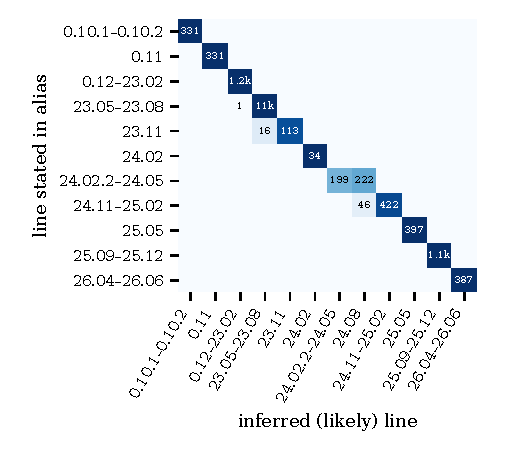
\includegraphics[width=\columnwidth]{figures/fig2_version_validation.pdf}
\caption{Release line stated in CLN developer aliases (rows) against the likely line inferred from feature bits
(columns), in node-days. Shading is the row share.}
\label{fig:validation}
\end{figure}

\begin{table}[t]
\centering\small
\caption{Validation against self-identifying aliases. Top: client labels of 797 nodes whose alias names their implementation. Bottom: release lines of CLN nodes whose alias states the running version, graded on every announced node-day.}
\label{tab:validation}
\begin{tabular}{lrrr}
\toprule
Client & Nodes & Precision (\%) & Recall (\%) \\
\midrule
LND & 664 & 100.0 & 96.4 \\
CLN & 117 & 98.3 & 99.1 \\
Eclair & 9 & 58.3 & 77.8 \\
LDK & 7 & 100.0 & 100.0 \\
\midrule
\multicolumn{3}{l}{CLN nodes / lines with a stated version} & 124 / 11 \\
\multicolumn{3}{l}{Node-days graded} & 15,549 \\
\multicolumn{3}{l}{Strict range contains the stated line (\%)} & 99.99 \\
\multicolumn{3}{l}{Likely line equals the stated line (\%)} & 98.2 \\
\multicolumn{3}{l}{Node--line pairs exact on every day} & 132 / 136 \\
\multicolumn{3}{l}{\quad 95\% CI (\%)} & [93, 99] \\
\bottomrule
\end{tabular}
\end{table}

